\section{X-ray crystallography}
Voraussetzung: regulären Kristall aus dem Protein\\
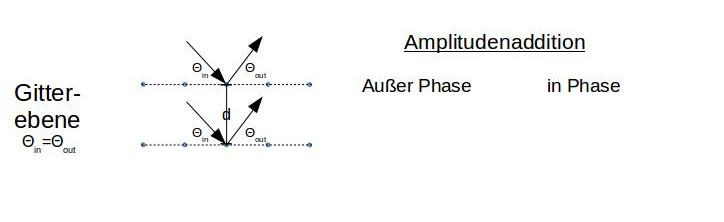
\includegraphics[width=1\textwidth]{lectures/160603/pix/1.jpg}
\textbf{Bragg's Law:} $n\lambda=2dsin(\Theta)$\\

\underline{X-ray crytallography diffraction:}\\
X-ray $\rightarrow$ Kristall $\rightarrow$ Ablenkung\\
durch Atome $\rightarrow$ Ablenkung wird durch einen Detektor gemessen\\
feste Wellenlänge $\lambda$, Winkel $\Theta$ variieren (Kristall rotieren) $\rightarrow$ charakteristisches Diffraction pattern $\rightarrow$ Amplitude ändert sich über den Winkel

$d_{hkl}=\frac{a_{0}}{\sqrt{h^2+k^2+l^2}}$ mit hkl=Laue-Index, $a_0=Gitterkonstante$
\\\\
oder:\\
$\Theta$ fest und $\lambda$ variiren $\rightarrow$ white x-ray\\
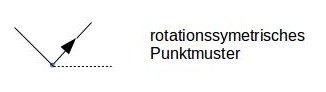
\includegraphics[width=0.5\textwidth]{lectures/160603/pix/2.jpg}
\\
Kombinierte Information aus allen Messungen für verschiedene $\lambda \& \Theta$
\\
\begin{enumerate}
	\item Backbone des Proteins ($COOH-NH_2$)
	\item Bestimmung der Position der flexiblen Seitenketten der Aminosäuren
	\item Verbesserung
\end{enumerate}

\section{NMR spectroscopy}
NMR: nuclear magnetic resonance\\
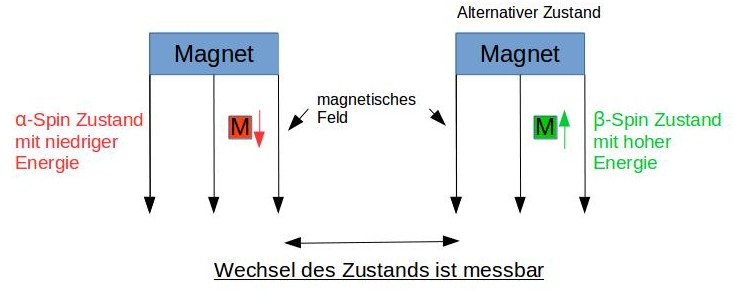
\includegraphics[width=1\textwidth]{lectures/160603/pix/3.jpg}

Atome mit magnetischen Eigenschaften: H, Deuterium, N, C, Li, B, O\\
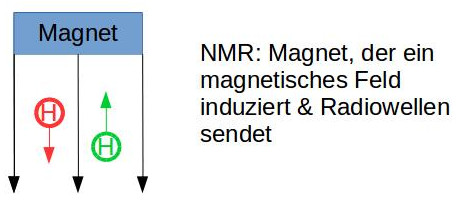
\includegraphics[width=0.5\textwidth]{lectures/160603/pix/4.jpg}

$\rightarrow$ ohne weitere äußere Einflüsse Atom in $\alpha-spin$\\
$\rightarrow$ über Flips im Magnetfeld Ermittlung der Protein-Struktur\\

Spektren von H,C,N + Strukturformel der bekannten Aminosäure + Aminosäureketten $\rightarrow$ Wechselwirkungen zwischen den Gruppen herleiten $\rightarrow$ 3D Koordinaten berechnen